\documentclass{article}
\usepackage[utf8]{inputenc}
\usepackage{graphicx}

\title{Othello AI Assignment}
\author{Jonathan Böcker}
\date{September 2016}

\usepackage{natbib}
\usepackage{graphicx}
\usepackage{listings}
\usepackage{color}
\usepackage[a4paper, margin=1in]{geometry}

\definecolor{codegreen}{rgb}{0,0.6,0}
\definecolor{codegray}{rgb}{0.5,0.5,0.5}
\definecolor{codepurple}{rgb}{0.58,0,0.82}
\definecolor{backcolour}{rgb}{0.95,0.95,0.92}

\lstdefinestyle{mystyle}{
    backgroundcolor=\color{backcolour},
    commentstyle=\color{codegreen},
    keywordstyle=\color{magenta},
    numberstyle=\tiny\color{codegray},
    stringstyle=\color{codepurple},
    basicstyle=\footnotesize,
    breakatwhitespace=false,
    breaklines=true,
    captionpos=b,
    keepspaces=true,
    numbers=left,
    numbersep=5pt,
    showspaces=false,
    showstringspaces=false,
    showtabs=false,
    tabsize=2
}


\lstset{style=mystyle}

\begin{document}

\maketitle

\section{Introduction}

This assignment consists of implementing the alpha-beta pruning search algorithm \citep{russel2010artifical}
and heuristic evaluation functions for an Othello AI opponent. I chose to implement
proper Othello rules and expand the board area to an 8 by 8 grid to make it a little
more challenging. I also chose to make the search algorithm with an iterative deepening search,
making it time dependent instead.
This makes the algorithm `smarter' the faster the host CPU is.

\section{Building the search algorithm}

I chose to represent the search nodes as states, that holds a snapshot of all important
variables at the time of evaluation. It is important to understand this class in order to understand
the search algorithm:

\begin{lstlisting}[language=Java]
class StateNode {
    private int[][] gridState;
    private int alpha = Integer.MIN_VALUE;
    private int beta = Integer.MAX_VALUE;
    private int player;
    private boolean isEndState = false;
    private int depth;
    private StateChange bestChange;
}
\end{lstlisting}

\begin{itemize}
\item The \verb|gridState| variable is an integer matrix where values span from -1 to 1,
where -1 represents a human player brick, 1 represents an AI brick and 0 represents
an unoccupied space. This is an application wide representation of the Othello board.

 \item The \verb|alpha| and \verb|beta| variables are important to the pruning algorithm at
every node to evaluate the need of searching further down in the current branch.

\item The \verb|player| int variable is either 1(AI) or -1(Human) and tells the algorithm
which player is about to make the next virtual draw in this node.

\item The \verb|isEndState| boolean variable is used to determine if a total board score
is relevant. This is important when the algorithm needs to know if the node is a
leafnode e.g. when the algorithm isn't allowed to search further due to time constraints.

\item The \verb|depth| int variable is only for requirements sake. It keeps
track of current search depth, making it possible to graphically display the search depth for the user.

\item The last instance variable \verb|bestChange| is an object with the following specifications:
\end{itemize}

\begin{lstlisting}[language=Java]
class StateChange {
    private StateNode endNode;
    private OthelloCoordinate move;
}
\end{lstlisting}

Its purpose is to keep track of the, according to the search algorithm, best state
change and by extension the best next draw for this node. This is most useful
for the root node when asked to provide the next AI draw. In this context the draw
is an object named move, simply holding a row and a column value in the board matrix as follows:
\begin{lstlisting}[language=Java]
class OthelloCoordinate {
    private int row;
    private int col;
}
\end{lstlisting}

\verb|StateNode| has one package-private constructor which is called when the application
controller wants a calculated draw from the AI:

\begin{lstlisting}[language=Java]
StateNode(int[][] gridState, OthelloController controller, long deadline){
      this.gridState = gridState;
      this.player = OthelloGUI.AI;
      this.depth = 0;
      controller.nodeFound(this.depth);
      findAllStateChanges(controller, deadline);
}
\end{lstlisting}

The constructor passes on the \verb|OthelloController| to the recursive method
\verb|findAllStateChanges()| after it has reported itself as a found node at depth 0.
One of the first things done in \verb|findAllStateChanges()| is checking if it should
attempt to find more nodes:

\begin{lstlisting}[language=Java]
private void findAllStateChanges(OthelloController controller, long deadline){
      ArrayList<StateChange> exploredChanges = new ArrayList<>();
      // Check if there is any limitations or we should keep looking
      if(this.shouldKeepLooking(deadline)) {
      ...
\end{lstlisting}

The method \verb|shouldKeepLooking()| has the purpose of limiting the search depth
according to some criteria, in this case it is a time limit:

\begin{lstlisting}[language=Java]
private boolean shouldKeepLooking(long deadline) {
        return System.currentTimeMillis() < deadline;
}
\end{lstlisting}

If \verb|shouldKeepLooking()| returns true, \verb|findAllStateChanges()| will continue to take
all possible draws and create a new \verb|StateNode| for each one using the private
constructor solely for recursive calls:

\begin{lstlisting}[language=Java]
private StateNode(int[][] gridState, int player, int alpha, int beta, int depth, OthelloController controller, long deadline)
\end{lstlisting}

The private constructor requires a little more information. The \verb|player|
variable oscillates between Human or AI between every recursive call in order for the
pruning algorithm to decide whether it is a prunable branch or not. The player variable
also controls if alpha or beta is passed back to the parent node when asked for its value.

\section{The pruning condition}

When looping through the matrix and exploring nodes in the current tree branch, there might be no need to
search further. Towards the end of the \verb|findAllStateChanges()| evaluation loop, the algorithm checks
and perhaps updates the alpha and beta values as follows:

\begin{lstlisting}[language=Java]
private void findAllStateChanges(OthelloController controller, long deadline){
...
// Check if we've found a prunable branch
  if (prune(change))
      break evaluationLoop;
\end{lstlisting}

It makes a call to \verb|prune()| with a calculated state change as the argument,
which returns \verb|true| or \verb|false| whether to cancel the search for more nodes.
The \verb|prune()| method looks as follows:

\newpage
\begin{lstlisting}[language=Java]
private boolean prune(StateChange change){
    int value = change.getEndNode().getValue();
    if(this.player == OthelloGUI.HUMAN && value <= beta) {
        beta = value;
        bestChange = change;
    } else if (this.player == OthelloGUI.AI && value >= alpha) {
        alpha = value;
        bestChange = change;
    }
    return this.player == OthelloGUI.HUMAN && this.alpha > this.beta ||
            this.player == OthelloGUI.AI && this.alpha < this.beta;
}
\end{lstlisting}

The pruning algorithms reasoning is that if the current node is AI, the child node
must be human. If that is so, it wants to see if the child nodes beta value is larger
than its own alpha value. Because if it is, that path of draws is the most favorable
for the moment, so it saves that draw and beta value as its alpha value until it finds a better one.

In the other way around, when the current node is human and child node is AI, it
checks if its child nodes alpha value is smaller than its beta.
If that is true it updates its beta to the child nodes alpha and saves the draw
as the most favorable draw. If the child node is a leaf node, it simply compares with the board score count.

Lastly, the condition that decides whether there is reason to keep looking in that branch,
is if the current node is AI and its alpha is larger than its beta. If that is true there is
no point in looking further into that branch.
In the other way around, if the node is human and its alpha is smaller than its beta, there is
no reason to continue in that branch.

\section{The evaluation functions}

There are several things to be evaluated in the Othello Game. The easiest and most crucial
is the board score, which is designed for the AI perspective. A positive score means that the
AI has more bricks on the board, a negative score means that the human player has more bricks
and a board score of zero means that the brick count is even. The static function for
calculating the board score is a simple nested for-loop that sums all integers in an integer
matrix representing the Othello board:

\begin{lstlisting}[language=Java]
static int boardScore(int[][] board) {
      int count = 0;
      for (int[] aBoard : board)
          for (int anABoard : aBoard) count += anABoard;
      return count;
}
\end{lstlisting}

This is possible due to the player representation I have chosen, where an AI brick is the
integer 1, and a human brick is -1. An unoccupied space is simply 0. This method is called
in the \verb|getValue()| method, which is called by the \verb|prune()| method.
The \verb|getValue()| method looks as follows:

\begin{lstlisting}[language=Java]
int getValue() {
        if(this.isEndState){
            return Utilities.boardScore(this.gridState);
        } else if(this.player == OthelloGUI.AI) {
            return this.alpha;
        } else {
            return this.beta;
        }
}
\end{lstlisting}

As stated in the pruning section, the algorithm makes some assumptions. If the current
node is AI, the parent node most probably wants the alpha value. Similarly if the current
node is human, the parent node wants the beta value. Leafnodes stands out, since there
is no point in returning alpha or beta. A leafnode represents an endgame and simply returns
the boardscore

How does the node know if it is a leafnode you might ask? Well, it might not be the end
of the game at all in the current node. It might pose as a leafnode if it is not allowed
to search further due to time constraints. It might be an endgame even if not all cells
in the grid are occupied, if neither the AI or the human player are able to make a move.

That leads us in to another evaluation function, \verb|findValidMoves()|. It takes
two arguments, the board matrix and the player about to make a move. It returns a
boolean matrix where \verb|true| values means there is a valid move. It loops through the matrix,
evaluating every position which is unoccupied, through calling the \verb|isValidMove()|
function. \verb|isValidMove()| checks in all 8 legal directions through calling the
\verb|possibleDirection()| function 8 times with different arguments.

\verb|possibleDirection()| is a somewhat complex function generalizing a direction check as follows:

\begin{lstlisting}[language=Java]
private static boolean possibleDirection(int deltaRow, int deltaCol, int row, int col, int[][] grid, int player) {
        int currentRow = row;
        int currentCol = col;

        if(currentRow + deltaRow < grid.length &&
                currentRow + deltaRow >= 0 &&
                currentCol + deltaCol < grid[0].length &&
                currentCol + deltaCol >= 0 &&
                grid[currentRow + deltaRow][currentCol + deltaCol] != -player) {
            return false;
        }

        currentCol += 2 * deltaCol;
        currentRow += 2 * deltaRow;

        while (currentCol < OthelloGUI.COLS && currentCol >= 0 &&
                    currentRow < OthelloGUI.ROWS && currentRow >= 0) {
            if(grid[currentRow][currentCol] == OthelloGUI.NONE ) {
               return false;
            } else if (grid[currentRow][currentCol] == player) {
                return true;
            }
            currentCol += deltaCol;
            currentRow += deltaRow;
        }

        return false;
}
\end{lstlisting}

The \verb|deltaRow| and \verb|deltaCol| parameters decides how big of a step, row-wise and column-wise,
the function should take every iteration in its while loop. The \verb|row| and \verb|col| parameters are
the draw to be examined, \verb|grid| and \verb|player| are self-explanatory.

Before anything else, the function checks to see if the intended draw has an opponent brick next to it,
one \verb|deltaCol| and \verb|deltaRow| away(line 5-11). If it does not, it is not a valid move and the function returns \verb|false|
immediately. If it does, it starts iterating in that direction to see if there is a brick belonging
to the intended player further away, with no unoccupied spaces inbetween(line 16-25). If it finds such a brick,
it is indeed a valid draw in that particular direction and the function returns \verb|true|(line 21). Although, if it finds
an unoccupied space before finding a player brick, it is not a valid move and returns \verb|false|(line 19).

Lastly, there is only one more important evaluation function. It takes a draw that is to be made and flips
as many bricks as possible on an Othello board according to Othello rules. The function is:

\begin{lstlisting}[language=Java]
static int[][] calculateBoardChange(int[][] start, OthelloCoordinate move, int player)
\end{lstlisting}

It is very similar to \verb|isValidMove()| in that it checks all 8 legal directions for bricks to flip.
It assumes it is a valid move to begin with and puts down the player brick before checking all the directions.
It calls a similar, but different function than \verb|isValidMove()| does, called \verb|lookInDirection()|.
\newpage

\begin{lstlisting}[language=Java]
private static int[][] lookInDirection(int deltaRow, int deltaCol,
        OthelloCoordinate move, int[][] grid, int player) {
    int currentRow = move.getRow() + deltaRow;
    int currentCol = move.getCol() + deltaCol;

    while (currentCol < OthelloGUI.COLS && currentCol >= 0 &&
              currentRow < OthelloGUI.ROWS && currentRow >= 0) {
        if(grid[currentRow][currentCol] == OthelloGUI.NONE) {
            break;
        } else if (grid[currentRow][currentCol] == player) {
            while (currentCol != move.getCol() || currentRow != move.getRow()) {
                grid[currentRow][currentCol] = player;

                currentCol -= deltaCol;
                currentRow -= deltaRow;
            }
            break;
        }
        currentCol += deltaCol;
        currentRow += deltaRow;
    }
    return grid;
}
\end{lstlisting}

It starts with looking in the \verb|deltaRow| and \verb|deltaCol| direction for a \verb|player| brick,
and aborts if it finds an unoccupied cell(line 8-9). When it finds a \verb|player| brick, it enters
a nested while-loop, iterating in the opposite direction and turning all bricks into \verb|player| bricks until
it is back to the original draw coordinate. It then breaks the outer while-loop, because the function has done
what it is supposed to.

Below is a UML class diagram summary of the program:

\begin{figure}[h]
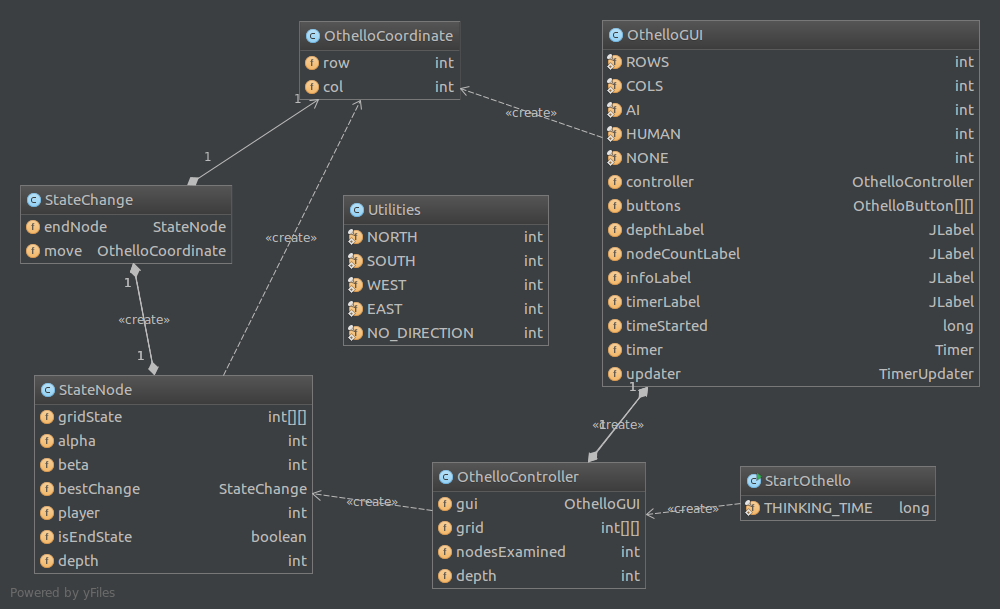
\includegraphics[width=\textwidth]{diagram.png}
\centering
\caption{A class diagram showing the class relationships of the program.}
\end{figure}

\newpage
\section{Discussion}
\subsection{If I had done it all over again}

The application was highly unoptimized at the time this paper was written, and I would
opt for a more object oriented approach when finding possible moves if I had to do
the assignment again. In the \verb|Utilities| class, there are three different methods
that could be combined in order to not iterate through the whole matrix several times.
Instead of returning a matrix with booleans in the \verb|findValidMoves()| method,
a list of coordinates would be preferrable. The list would then deprecate methods such
as \verb|numberOfValidMoves()| and \verb|hasValidMoves()|, because a list already contains
such information.
This would of course increase the performance and make a better AI on slow systems.

I would also cut down on dependencies such as the \verb|OthelloCoordinate| class,
since it could easily be replaced by an int array of two elements. Another class that
showed little to no use was \verb|StateChange|, which I thought would be handy when
creating a state transition table if I had the time.

To make the source code more clear, and to make it more readable for a person
familiar with the minimax algorithm, I would follow the pseudo code more closely.
At the time of writing, there is no mention of the \verb|Max-Value()| and \verb|Min-Value()|
methods in the source code, which may confuse the reader. The implementation may even be
wrong at places. This is because I thought I would be able to make a shorter and a more
compressed solution, and it would be more clear to approach the algorithm with a
human/AI approach instead of a min/max approach.

\subsection{Experiences}

All in all, I gained lots of experience during this assignment. It is the first time
I've constructed an application able to slow down a graphical interface in such a way
it was noticeable when not using thread workers. This lead me into researching and learning
about Java Swings \verb|SwingWorker| class and the usefulness of the \verb|SwingUtilities.invokeLater()|
method. This prevented the graphical user interface from freezing when the AI was calculating
the next move.

I found the mini-max with alpha-beta pruning algorithm very interesting and a great introduction
to what may be considered an intelligent system. I realize it may be flawed and not be
optimal to this application, but it was comprehensible and educational enough for me to
be able to grasp more sophisticated algorithms in the same problem domain.

I now realize that some problems may not be feasible to solve perfectly due to the
complexity in some cases. A similar application for a different game e.g. the game of Go\citep{alphago},
the time complexity would be to large with this algorithm.

I tried to implement a state transition table in order to store comuted nodes in the tree and failed,
as it was to complex for me to re-implement methods such as \verb|hashCode()| and \verb|equals()| in the keys
to the hashmap. The re-implementation would be necessary to be able to fetch the stored
objects in a hashmap with a newly constructed key. Another challenge was to sort out what information to store
in the table, as some information was time dependant and other was changed from search to search, such
as the alpha/beta values. This is a valuable experience, and it would be interesting to see if
there would be any computational gains to store objects in such fashion.


\bibliographystyle{plain}
\bibliography{references}

\end{document}
